\documentclass[10pt,twocolumn]{article}

\usepackage[T1]{fontenc}
\usepackage[utf8]{inputenc}
\usepackage[margin=0.74in]{geometry}
\usepackage{amsmath}
\usepackage{booktabs}
\usepackage{graphicx}
\usepackage{microtype}
\usepackage{enumitem}
\usepackage[hidelinks]{hyperref}
\usepackage[numbers,sort&compress]{natbib}
\usepackage{caption}
\captionsetup{font=small,labelfont=bf}

\newcommand{\task}[1]{\texttt{#1}}
\newcommand{\model}[1]{\textsc{#1}}
\setlist[itemize]{leftmargin=*,nosep}
\setlength{\parskip}{2pt}
\setlength{\parindent}{10pt}

\title{\vspace{-1.3em}\textbf{SUPERCUTE: From Tokenizer Friction to Model-Specific Long-Horizon Breaks}}
\author{Stanislav Kirdey\\Clark Labs Inc.\\\texttt{stan@clarkslabs.com}}
\date{June 2026}

\begin{document}
\twocolumn[
\maketitle
\begin{center}
\begin{minipage}{0.92\textwidth}
\small
\noindent\textbf{Abstract.}
Many character-level benchmarks assume that tokenizer friction is the main weakness of large language models. SUPERCUTE tests that assumption with deterministic, exactly graded tasks. We evaluate six reasoning-enabled models on three scored tiers: tokenizer perception probes, realistic tokenizer-sensitive workflows, and a controlled long-horizon execution stress test. We also release PublicLift, an unscored set of public-dataset-derived hardening templates. In this pilot run, tokenizer perception does not reliably break GPT-5.5: it scores 149/152 on probes involving homoglyphs, zero-width characters, Unicode normalization, code points, UTF-8 byte length, and grapheme operations. Realistic mutable workflows are harder: GPT-5.5 scores 50/64, while the weakest model scores 14/64. The controlled \task{iterated\_lut} tier shows a model-specific long-horizon break: GPT-5.5 falls from 7/8 at 330 interdependent updates to 0/8 at 1320 updates, but Claude Opus 4.8 scores 33/40 overall and reaches 8/8 at the same 1320-update setting. Thus the evidence does not support a universal frontier wall. It supports a narrower claim: isolated tokenizer perception is a weak stressor for GPT-5.5, while exact execution over long mutable state produces high-variance, model-dependent failures that require larger sweeps and token-budget-controlled comparisons.
\vspace{0.6em}
\end{minipage}
\end{center}
\vspace{0.5em}
]

\section{Introduction}
Character-level errors matter in everyday work. A single invisible character can change a customer ID. A confusable letter can split an invoice group. A line number in a patch can shift after one edit. A contract amendment can refer to a clause by a visually similar but distinct identifier. Earlier tokenizer-focused work, such as CUTE \citep{edman2024cute}, made this problem concrete by asking whether language models can reason about the characters inside their tokens. Recent work such as CharBench \citep{uzan2026charbench} continues to show that character-level counting and position tasks remain hard for many models.

This paper asks a narrower question: what still fails when a frontier reasoning model is allowed to think at length? Our answer is intentionally cautious. Static tokenization probes are mostly solved by GPT-5.5 in our run. The stronger stressor is exact execution over mutable state: many small updates, no algebraic shortcut, and a high-entropy final answer. But this is not a universal frontier failure. On the controlled LUT task, GPT-5.5 fails sharply at longer horizons while Opus 4.8 remains much stronger. The interesting signal is therefore model-specific reliability, not a single leaderboard claim.

SUPERCUTE is designed to expose this boundary while keeping the evaluation auditable. Every task has deterministic ground truth. The grader accepts exact answers and robustly extracts final answers from verbose model responses. The benchmark avoids manual judging for its core score. It also avoids tasks that are hard only because they require tools, such as computing a cryptographic hash.

We make four contributions:
\begin{itemize}
  \item A negative result: tokenizer perception is near-saturated for GPT-5.5 on our battery.
  \item RealTok: eight realistic exact-state workflows that place tokenizer-sensitive details inside human-relevant work.
  \item A controlled pilot break curve for shortcut-free full-state execution, plus a simple compounding-error fit.
  \item PublicLift: released templates for turning finance tables, contracts, receipts, logs, code traces, software patches, and spreadsheets into fresh exact-state tasks. These templates are not scored in the supplied run.
\end{itemize}

\section{Related Work}
\paragraph{Tokenizer and character understanding.}
CUTE tests whether models can manipulate characters despite operating over tokens \citep{edman2024cute}. CharBench scales this idea and separately studies occurrence tracking and positional understanding \citep{uzan2026charbench}. Byte-level or patch-level architectures such as BLT attempt to reduce dependence on fixed token boundaries \citep{pagnoni2024blt}. SUPERCUTE differs by asking when a reasoning model that can solve isolated character probes still fails in exact workflows.

\paragraph{Long-horizon execution.}
Several recent studies argue that long tasks fail because small errors compound. The Illusion of Diminishing Returns studies long-horizon execution and shows that single-step quality can turn into task-length limits \citep{herel2025illusion}. Work on finite-state-machine execution isolates state maintenance over long horizons \citep{fsm2025procedural}. Long-context benchmarks such as RULER and NoLiMa show that retrieval-like success is not enough when lexical overlap, multi-hop tracing, and aggregation become harder \citep{hsieh2024ruler,keren2025nolima}. SUPERCUTE focuses on exact mutable state rather than broad QA.

\paragraph{Real-world substrates.}
Public datasets offer realistic records and automatic or semi-automatic oracles. FinQA and TAT-QA use financial reports and tables \citep{chen2021finqa,zhu2022tatqa}; TabFact and WikiTableQuestions use semi-structured tables \citep{chen2020tabfact,pasupat2015wikitq}; SpreadsheetBench is built from real spreadsheet problems \citep{ma2024spreadsheetbench}; CRUXEval tests code execution and input/output reasoning \citep{gu2024cruxeval}; SWE-bench evaluates patches for real GitHub issues \citep{jimenez2024swebench}; CUAD and ContractNLI cover legal contracts \citep{hendrycks2021cuad,koreeda2021contractnli}; CORD and DocVQA cover document and receipt extraction \citep{park2019cord,mathew2021docvqa}; LogHub collects real system logs \citep{zhu2023loghub}. PublicLift uses these datasets as substrates, not as static questions.

\section{Benchmark Design}
SUPERCUTE uses generators rather than fixed puzzles. A generator receives a random seed and returns a prompt, answer, kind, and metadata. This gives fresh variants, exact ground truth, and cheap self-checking.

\subsection{Core requirements}
A task is included only if it meets four requirements.
\begin{itemize}
  \item \textbf{Exact oracle.} The answer is computed by deterministic code.
  \item \textbf{No hidden tool dependency.} A model should not need a calculator, code interpreter, or web browser.
  \item \textbf{No easy shortcut in the hard tier.} Linear rules, last-write-wins fields, and single accumulators are useful diagnostics but not final breakers.
  \item \textbf{Realistic contact point.} In RealTok and PublicLift, the hard detail should look like work a person might delegate: merging redlines, replaying patches, cleaning receipts, reconciling ledgers, or auditing logs.
\end{itemize}

\subsection{Scored tiers}
\paragraph{Tok.}
The tokenizer perception tier includes 19 tasks: homoglyph counting and localization, zero-width characters, combining marks, Unicode normalization, case-folding expansion, astral code points, code point and UTF-8 byte reporting, confusable digits, large-number digit operations, grapheme segmentation, and related probes.

\paragraph{RealTok.}
RealTok includes eight realistic exact-state workflows. Examples include reconstructing a CRM field from cursor edits, applying a ticket-board JSON patch stream, cleaning a Unicode-noisy invoice CSV, auditing synthetic redaction leaks, merging contract redlines, reconciling warehouse scans, reconstructing a clinical sequence, and merging localization strings.

\paragraph{LUT.}
The \task{iterated\_lut} tier is a controlled stress test. It samples a random $10\times10$ transition table $T$ and a digit string $s$ of width $L=22$. Each round applies
\[
    s'_{i} = T[s_i][s_{i+1}],
\]
with wraparound. We vary the number of rounds $K\in\{15,30,45,60,75\}$, giving 330 to 1650 interdependent cell updates. Because $T$ is random and the whole state changes, the task has no known simple closed form. Since $L$ is fixed in the supplied run, this is a depth sweep, not a two-dimensional width-by-depth study.

\paragraph{PublicLift release tier.}
PublicLift is released infrastructure, not scored evidence in this paper. It provides hardened templates for public data records. The public record supplies realism; a seeded changelog supplies freshness and anti-contamination; a Python oracle supplies the exact label. The templates intentionally do not redistribute third-party rows.

\section{Experimental Setup}
We evaluated six reasoning-enabled models through OpenRouter in June 2026: GPT-5.5, Claude Opus 4.8, DeepSeek V4 Pro, MiniMax M3, Qwen 3.7 Plus, and Qwen 3.5 Flash. Temperature was set to 0. The Tok and RealTok tiers use $n=8$ variants per task. The LUT break curve uses $n=8$ variants for each model and each value of $K$. We report exact-match accuracy and Wilson 95\% confidence intervals.

The raw run contains 1536 model calls. Thirteen provider or transport errors are kept in the raw JSONL but dropped from scored denominators, leaving 1523 scored rows. This explains denominators such as 33/62 and 4/37. Tables report scored denominators, and the release preserves the dropped-error counts.

The grader first looks for explicit answer markers and otherwise extracts the final answer-like span from the end of the response. This matters because reasoning models often produce long explanations before the final answer. We validated the extractor against raw model outputs before scoring. A free self-check verifies that every generator's own answer is accepted by both the strict and robust grader.

Reasoning budget is a major confound. Models expose and use reasoning tokens differently, and some providers report hidden reasoning separately while others mainly expose total completion tokens. We therefore report token counts for the LUT tier and interpret within-model curves as more stable than cross-model rankings. Even the within-model curve should be treated as a pilot because $n=8$ per cell is small.

\section{Results}
\subsection{Finding 1: tokenizer perception is mostly solved for GPT-5.5}
Table~\ref{tab:tok} shows the Tok tier. GPT-5.5 solves 149 of 152 items. The remaining errors are not concentrated in Unicode perception. They appear in long-run counting and related static exactness tasks. This means isolated tokenizer friction is not enough to break the strongest model in our run.

\begin{table}[t]
\centering
\small
\begin{tabular}{lrrr}
\toprule
Model & Correct & Acc. & 95\% CI \\
\midrule
GPT-5.5 & 149/152 & 0.980 & [0.944, 0.993] \\
DeepSeek V4 Pro & 136/152 & 0.895 & [0.836, 0.934] \\
Qwen 3.7 Plus & 131/152 & 0.862 & [0.798, 0.908] \\
MiniMax M3 & 129/152 & 0.849 & [0.783, 0.897] \\
Opus 4.8 & 128/152 & 0.842 & [0.776, 0.892] \\
Qwen 3.5 Flash & 121/152 & 0.796 & [0.725, 0.852] \\
\bottomrule
\end{tabular}
\caption{Tokenizer perception tier. These probes stratify models, but they do not break GPT-5.5 in this run.}
\label{tab:tok}
\end{table}

\subsection{Finding 2: realistic mutable workflows are harder}
Table~\ref{tab:realtok} shows the RealTok tier. The same kinds of character details become harder when they are part of a task with mutable state. GPT-5.5 remains best, but drops to 50/64. Qwen 3.5 Flash falls to 14/64.

\begin{table}[t]
\centering
\small
\begin{tabular}{lrrr}
\toprule
Model & Correct & Acc. & 95\% CI \\
\midrule
GPT-5.5 & 50/64 & 0.781 & [0.666, 0.865] \\
DeepSeek V4 Pro & 33/62 & 0.532 & [0.410, 0.651] \\
Opus 4.8 & 33/63 & 0.524 & [0.403, 0.642] \\
MiniMax M3 & 25/61 & 0.410 & [0.295, 0.535] \\
Qwen 3.7 Plus & 20/60 & 0.333 & [0.227, 0.459] \\
Qwen 3.5 Flash & 14/64 & 0.219 & [0.135, 0.334] \\
\bottomrule
\end{tabular}
\caption{RealTok tier. Tokenizer-sensitive details are embedded in realistic exact-state work. Denominators below 64 reflect dropped provider/transport errors.}
\label{tab:realtok}
\end{table}

The hardest RealTok tasks are edit replay tasks. CRM field reconstruction scores 2/8 for GPT-5.5 and 0/8 for every other model. Legal redline merge scores 3/8 for GPT-5.5, 2/8 for Opus, and 0/8 for the other models. This is consistent with the hypothesis that moving cursors, shifting positions, and preserving exact text create many chances for small errors.

One RealTok task is intentionally instructive: \task{json\_patch\_ticket\_board} is easy for every model. Most fields are last-write-wins, so a model can skip much of the history. This is a design warning. A hard benchmark needs full-state updates that resist compression.

\subsection{Finding 3: LUT exposes model-specific long-horizon failures}
Figure~\ref{fig:breakcurve} and Table~\ref{tab:lut} show the LUT break curve. GPT-5.5 falls sharply as the number of interdependent updates increases: 7/8 at $K=15$, 4/8 at $K=30$, 3/8 at $K=45$, 0/8 at $K=60$, and 1/8 at $K=75$. These are complete answers with normal stop reasons, not truncated outputs.

However, the curves are not monotonic and the cells are small. GPT-5.5 goes from 0/8 at $K=60$ back to 1/8 at $K=75$, while Opus dips to 6/8 at $K=45$ and recovers to 8/8 at $K=60$. The correct interpretation is not ``longer always lowers accuracy'' from these $n=8$ cells. It is that random full-state execution produces noisy but visible model-specific reliability differences.

\begin{figure*}[t]
\centering
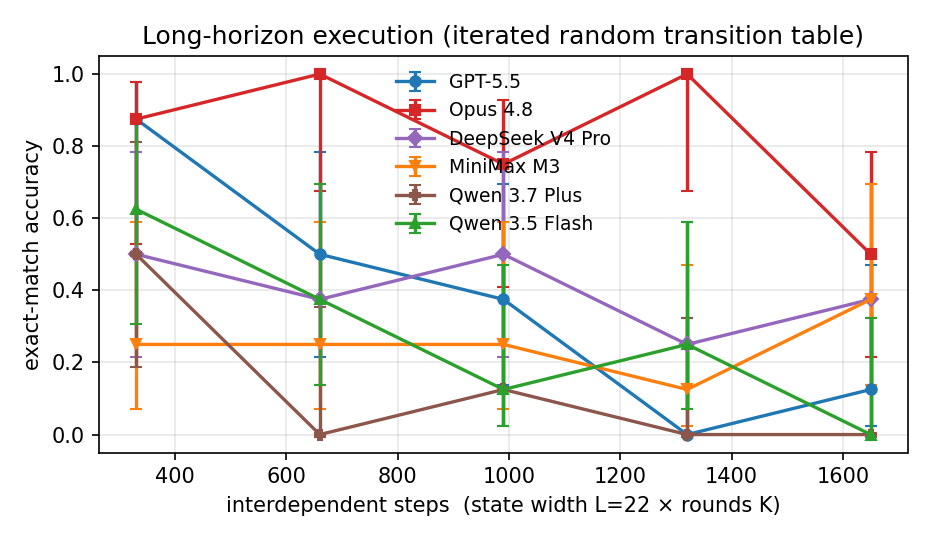
\includegraphics[width=0.76\linewidth]{figures/breakcurve.png}
\caption{Long-horizon execution pilot for \task{iterated\_lut}. The x-axis is $22\times K$ interdependent updates. Error bars are Wilson 95\% intervals. The jagged curves show why larger $n$ is needed before drawing fine-grained ordering claims.}
\label{fig:breakcurve}
\end{figure*}

\begin{table}[t]
\centering
\small
\begin{tabular}{lrrr}
\toprule
Model & Correct & Acc. & 95\% CI \\
\midrule
Opus 4.8 & 33/40 & 0.825 & [0.680, 0.913] \\
DeepSeek V4 Pro & 16/40 & 0.400 & [0.263, 0.554] \\
GPT-5.5 & 15/40 & 0.375 & [0.242, 0.530] \\
Qwen 3.5 Flash & 11/40 & 0.275 & [0.161, 0.428] \\
MiniMax M3 & 10/40 & 0.250 & [0.142, 0.402] \\
Qwen 3.7 Plus & 4/37 & 0.108 & [0.043, 0.247] \\
\bottomrule
\end{tabular}
\caption{Overall LUT accuracy across $K\in\{15,30,45,60,75\}$. Qwen 3.7 Plus has three dropped provider/transport errors, giving 37 scored calls.}
\label{tab:lut}
\end{table}

The result is also entangled with reasoning budget. At $K=60$, GPT-5.5 averages about 16.8k completion tokens and scores 0/8. Opus averages about 34.8k completion tokens and scores 8/8. GPT-5.5's token use rises from $K=15$ to $K=45$ and then nearly plateaus, while Opus completion length continues to grow with $K$. But budget alone cannot explain all results: Qwen 3.5 Flash reaches about 87k completion tokens at $K=75$ and still scores 0/8. The safer conclusion is that token budget and per-step precision interact.

\subsection{A simple compounding-error fit}
The long-horizon framing predicts that final exact accuracy should decay as small execution errors accumulate. To summarize the jagged curves, we fit the one-parameter model
\[
    P(\text{correct}\mid K,m) = r_m^K = q_m^{22K},
\]
where $r_m$ is fitted per-round survival for model $m$ and $q_m$ is the equivalent per-cell-update survival under fixed $L=22$. This is a descriptive binomial maximum-likelihood fit, not evidence that errors are independent.

\begin{table}[t]
\centering
\scriptsize
\setlength{\tabcolsep}{3pt}
\begin{tabular}{lrrr}
\toprule
Model & $r$ & $q$ & half upd. \\
\midrule
Opus 4.8 & 0.9956 & 0.999800 & 3459 \\
DeepSeek V4 Pro & 0.9790 & 0.999034 & 717 \\
GPT-5.5 & 0.9739 & 0.998798 & 576 \\
MiniMax M3 & 0.9690 & 0.998572 & 485 \\
Qwen 3.5 Flash & 0.9659 & 0.998422 & 439 \\
Qwen 3.7 Plus & 0.9359 & 0.996993 & 230 \\
\bottomrule
\end{tabular}
\caption{Descriptive fit of $P(\mathrm{correct}|K)=r^K$ on the LUT tier. Here $r$ is fitted per-round survival, $q$ is equivalent per-update survival, and ``half upd.'' is the fitted half-life in cell updates.}
\label{tab:fit}
\end{table}

The fit clarifies the model-specific story. Opus has a much longer fitted half-life than GPT-5.5 on this task, which is consistent with its 33/40 overall score. GPT-5.5 is not the best model on LUT despite being strongest on Tok and RealTok. This undercuts any universal claim that all frontier models share the same long-horizon wall.

\section{PublicLift: Using Public Data to Go Harder}
Public datasets are useful, but reusing their original questions is not enough. Many original labels are low entropy, contaminated, or answerable by retrieval. PublicLift uses a procedural lift:
\[
    \text{public record} + \text{fresh changelog} \rightarrow \text{new exact-state task}.
\]
The changelog is generated at evaluation time. It contains realistic operations, Unicode-confusable identifiers, and many state updates. The oracle replays the same operations in Python and emits the final answer. In this paper PublicLift should be read as a release contribution and future evaluation direction, not as a scored result.

\begin{table*}[t]
\centering
\small
\begin{tabular}{lll}
\toprule
PublicLift task & Public substrate family & Exact target \\
\midrule
\task{finqa\_restatement\_rollforward} & FinQA, TAT-QA, MultiHiertt & final segment totals in cents \\
\task{tabfact\_table\_changelog} & TabFact, WikiTableQuestions, SpreadsheetBench & final requested rows \\
\task{cuad\_amendment\_merge} & CUAD, ContractNLI, LEDGAR & final clause text \\
\task{cord\_receipt\_reconciliation} & CORD, SROIE, DocVQA & final category totals \\
\task{loghub\_incident\_replay} & LogHub and AIOps logs & sorted open incidents \\
\task{cruxeval\_stack\_trace} & CRUXEval, LiveCodeBench, CodeNet & final stack \\
\task{swebench\_patch\_manifest} & SWE-bench and software patches & final line snapshots \\
\task{spreadsheet\_cell\_reconciliation} & SpreadsheetBench & final cell values and checksums \\
\bottomrule
\end{tabular}
\caption{PublicLift templates released with SUPERCUTE. These are designed to be fed by public records without redistributing third-party data.}
\label{tab:publiclift}
\end{table*}

This design makes the benchmark harder and more realistic. A finance task becomes a restatement rollforward, not a single table question. A contract task becomes an amendment merge, not clause classification. A receipt task becomes OCR correction and reconciliation, not one-field extraction. A software task becomes current-line patch replay, not only issue summarization. PublicLift gives the benchmark a path from controlled synthetic stress tests to human-relevant work, but it still needs a paid multi-model sweep before becoming an empirical claim.

\section{Code Release}
The release is organized as a normal Python package. It includes a registry of scenario generators, an OpenAI-compatible API client, strict and robust graders, sweep and benchmark runners, public-data adapter skeletons, analysis scripts, tests, CI, and documentation. The package has no required runtime dependencies beyond the Python standard library. Optional extras support plotting, datasets, and development.

The release commands are deliberately short. Run \task{python -m supercute.selfcheck} for the full local oracle check. Module-level self-checks use \task{python -m supercute.sweep --module <name> --self}, where \task{<name>} can be \task{tok}, \task{realtok}, \task{hard}, or \task{publiclift}. A paid model sweep only requires an OpenAI-compatible endpoint and API key. The full evaluation harness can optionally write raw prompts, oracle answers, and model responses for manual failure analysis.

\section{Limitations and Next Experiments}
The supplied model results come from one provider route and one time window. Reasoning models are not fully deterministic, even at temperature 0. Reasoning budgets differ across models and endpoints, so absolute cross-model rankings should be read with token spend. The LUT cells use only $n=8$, which makes the break curves jagged and the Wilson intervals wide. A convincing follow-up should use at least 30 to 50 variants per cell.

The LUT sweep fixes width $L=22$ and varies depth $K$, so it cannot identify whether width or depth is the dominant driver. A two-dimensional $L\times K$ grid is needed. We also do not include a human baseline. That matters because some RealTok tasks are framed as delegated work; the benchmark should verify that trained humans can complete representative items reliably with enough time. Finally, exact-match grading is intentionally strict. The supplied scored JSONL does not include raw responses, so this paper cannot provide a full failure taxonomy. The revised release adds an optional raw-output audit path for future runs.

\section{Conclusion}
SUPERCUTE started as a tokenizer-friction benchmark, but the supplied data point to a narrower and more useful claim. Isolated tokenizer perception is largely solved for GPT-5.5 in this run. Realistic exact-state workflows are harder. A random full-state LUT task reveals sharp failures for some models, including GPT-5.5, but not for all frontier models: Opus is much stronger on the same tier. The benchmark lesson is therefore practical rather than universal: measure exact state updates, remove shortcuts, report denominators and token budgets, and treat long-horizon execution as a model-specific reliability problem.

\section*{Reproducibility Statement}
The released artifact contains source code, raw supplied results, summary tables, the figure generator, tests, CI configuration, and this LaTeX source. Core tasks are deterministic and self-checkable without model calls. The raw supplied results include provider/transport errors so denominator choices can be audited.

\begin{thebibliography}{99}\small
\bibitem[Edman et~al.(2024)]{edman2024cute} Edman, L., Schmid, H., and Fraser, A. CUTE: Measuring LLMs' understanding of their tokens. EMNLP, 2024.
\bibitem[Uzan and Pinter(2026)]{uzan2026charbench} Uzan, O. and Pinter, Y. CharBench: Evaluating the role of tokenization in character-level tasks. AAAI, 2026.
\bibitem[Pagnoni et~al.(2024)]{pagnoni2024blt} Pagnoni, A. et al. Byte Latent Transformer: Patches scale better than tokens. arXiv:2412.09871, 2024.
\bibitem[Herel et~al.(2025)]{herel2025illusion} Herel, D. et al. The illusion of diminishing returns: Measuring long-horizon execution in LLMs. arXiv:2509.09677, 2025.
\bibitem[Anonymous(2025)]{fsm2025procedural} Anonymous. The illusion of procedural reasoning: Evaluating LLMs' long-horizon execution of finite state machines. arXiv:2511.14777, 2025.
\bibitem[Hsieh et~al.(2024)]{hsieh2024ruler} Hsieh, C.-P. et al. RULER: What's the real context size of your long-context language models? COLM, 2024.
\bibitem[Keren et~al.(2025)]{keren2025nolima} Keren, N. et al. NoLiMa: Long-context evaluation beyond literal matching. arXiv:2502.05167, 2025.
\bibitem[Kulagin et~al.(2025)]{kulagin2025tokenbreak} Kulagin, E. et al. TokenBreak: Advancing text classification attack by token manipulation. arXiv:2506.07948, 2025.
\bibitem[Chen et~al.(2021)]{chen2021finqa} Chen, Z. et al. FinQA: A dataset of numerical reasoning over financial data. EMNLP, 2021.
\bibitem[Zhu et~al.(2021)]{zhu2022tatqa} Zhu, F. et al. TAT-QA: A question answering benchmark on a hybrid of tabular and textual content in finance. AAAI, 2021.
\bibitem[Chen et~al.(2020)]{chen2020tabfact} Chen, W. et al. TabFact: A large-scale dataset for table-based fact verification. ICLR, 2020.
\bibitem[Pasupat and Liang(2015)]{pasupat2015wikitq} Pasupat, P. and Liang, P. Compositional semantic parsing on semi-structured tables. ACL, 2015.
\bibitem[Ma et~al.(2024)]{ma2024spreadsheetbench} Ma, Z. et al. SpreadsheetBench: Towards challenging real world spreadsheet manipulation. NeurIPS, 2024.
\bibitem[Gu et~al.(2024)]{gu2024cruxeval} Gu, A. et al. CRUXEval: A benchmark for code reasoning, understanding and execution. ICML, 2024.
\bibitem[Jimenez et~al.(2024)]{jimenez2024swebench} Jimenez, C. E. et al. SWE-bench: Can language models resolve real-world GitHub issues? ICLR, 2024.
\bibitem[Hendrycks et~al.(2021)]{hendrycks2021cuad} Hendrycks, D., Burns, C., Chen, A., and Ball, S. CUAD: An expert-annotated NLP dataset for legal contract review. NeurIPS Datasets and Benchmarks, 2021.
\bibitem[Koreeda and Manning(2021)]{koreeda2021contractnli} Koreeda, Y. and Manning, C. D. ContractNLI: A dataset for document-level natural language inference for contracts. Findings of EMNLP, 2021.
\bibitem[Park et~al.(2019)]{park2019cord} Park, S. et al. CORD: A consolidated receipt dataset for post-OCR parsing. NeurIPS Workshop on Document Intelligence, 2019.
\bibitem[Mathew et~al.(2021)]{mathew2021docvqa} Mathew, M., Karatzas, D., and Jawahar, C. V. DocVQA: A dataset for VQA on document images. WACV, 2021.
\bibitem[Zhu et~al.(2023)]{zhu2023loghub} Zhu, J. et al. Loghub: A large collection of system log datasets for AI-driven log analytics. ISSRE, 2023.
\end{thebibliography}

\end{document}
